\chapter{Principal Pipeline Components}
\label{chap:pipeline}

\section{Crawler and PDF Sources}
Scrapy crawls only configured and authorised targets, obeys robots.txt and uses conservative delays. HTML pages, RSS/Atom feeds and PDFs are dispatched through the same provenance-aware parser. PDF text is extracted with \texttt{pypdf}; short or failed extractions are rejected or recorded as failures.

\begin{figure}[H]
\centering
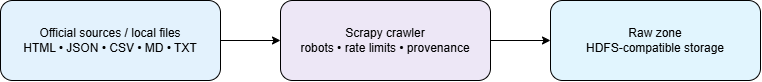
\includegraphics[width=0.9\textwidth]{images/01-ingestion.png}
\caption{Source ingestion and crawler flow.}
\label{fig:ingestion}
\end{figure}

\section{Raw Storage and ETL}
The raw zone writes to WebHDFS when enabled and falls back to local storage when the namenode is unavailable. Spark performs deduplication, whitespace normalization, source-domain normalization and minimum-text validation. A pure-Python ETL path remains available for local testing.

\begin{figure}[H]
\centering
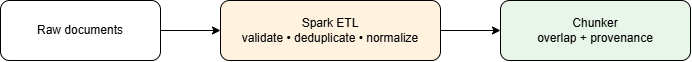
\includegraphics[width=0.9\textwidth]{images/02-etl-chunking.png}
\caption{ETL, validation and chunking stages.}
\label{fig:etl-chunking}
\end{figure}

\section{Chunking and Embeddings}
Validated pages are divided into overlapping text chunks using an 800-character window and 120-character overlap. The resulting step is 680 characters, which preserves context across boundaries. NVIDIA's embedding model \texttt{nvidia/nemotron-3-embed-1b} indexes the chunks in Qdrant. The offline deterministic test fallback uses 256 dimensions; production Qdrant collections take the dimension returned by the NVIDIA endpoint.

\section{BM25 and Hybrid Retrieval}
Retrieval combines cosine similarity from embeddings with BM25 lexical relevance. BM25 uses $k_1=1.2$, $b=0.75$ and a lexical multiplier of 2.2, with inverse document frequency computed over the indexed chunks and document-length normalization against the average chunk length. This hybrid score helps preserve exact names, acronyms and French/Arabic terms that may be missed by semantic similarity alone.

\section{Entity and Relation Extraction}
Mistral is used to extract typed entities and relations from chunks. The graph stores provenance through page and chunk links. A heuristic fallback, durable retry queue and extraction cache make failures visible without silently losing records.

\begin{figure}[H]
\centering
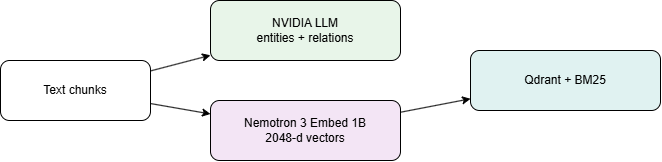
\includegraphics[width=0.9\textwidth]{images/03-extraction-embeddings.png}
\caption{Entity extraction and embedding generation.}
\label{fig:extraction-embeddings}
\end{figure}

\section{GraphRAG API and Frontend}
FastAPI exposes grounded questions, graph analytics, source pagination, PDF viewing, pipeline status and evaluation statistics. The React frontend provides the assistant conversation, source pages, graph explorer, operational pipeline view and evaluation dashboard.

\begin{figure}[H]
\centering
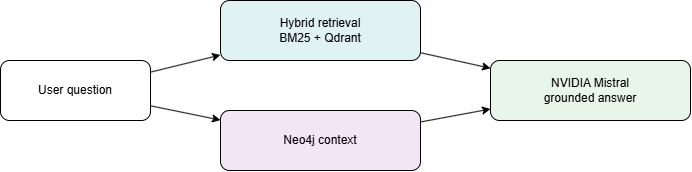
\includegraphics[width=0.9\textwidth]{images/05-graphrag-api.png}
\caption{GraphRAG API and retrieval flow.}
\label{fig:graphrag-api}
\end{figure}
